%------------------------------------------%
% Cannabis Data Science #128
% Copyright (c) 2022 Cannlytics
% Date: 9/27/2023
%------------------------------------------%
\documentclass[xcolor={dvipsnames}]{beamer}
\hypersetup{pdfpagemode = FullScreen}
\mode<presentation>{
  \usetheme{Boadilla}
  \usecolortheme{orchid}
  \usefonttheme{default}
  \setbeamertemplate{navigation symbols}{}
  \setbeamertemplate{caption}[numbered]
}
\setbeamersize{
  text margin left = 0.5in,
  text margin right = 0.5in
}

%------------------------------------------%
% Title
%------------------------------------------%
\title[\textbf{Cannabis Data Science \#128}]{}
\author{Cannlytics}
\institute[]{\Large Cannabis Data Science \#128}
\date{September \nth{27}, 2023}

%------------------------------------------%
% Packages
%------------------------------------------%
\usepackage[english]{babel}
\usepackage[utf8x]{inputenc}
\usepackage{tikz} % For styling.
\usepackage{xparse}
\usepackage{amsmath}
\renewcommand*\footnoterule{} % No footnote line.
\usepackage{mathtools} % Annotating equations.
\usepackage{hhline} % Double bars.
\usepackage[super]{nth} % 1st, 2nd, 3rd, etc.
\usepackage{graphicx, caption, subcaption}
\usepackage{setspace}
\usepackage[charter]{mathdesign}
\usepackage{tikz}
\usetikzlibrary{tikzmark}
\usetikzlibrary{arrows.meta}

%------------------------------------------%
% Theme
%------------------------------------------%
\definecolor{LG}{RGB}{218, 247, 166}
\definecolor{DG}{RGB}{2, 48, 32}
\setbeamercolor*{palette primary}{bg=LG, fg=DG}
\setbeamercolor*{palette secondary}{bg=LG, fg=DG}
\setbeamercolor*{palette tertiary}{bg=LG, fg=DG}

%------------------------------------------%
% Commands
%------------------------------------------%

% Top space.
\newcommand\T{\rule{0pt}{2.5ex}}

% Bottom space.
\newcommand\B{\rule[-1.25ex]{0pt}{0pt}}

% Blocks.
\newenvironment<>{Block}[2][.9\textwidth]
  {\setlength{\textwidth}{#1}
  \begin{actionenv}#3
    \def\insertblocktitle{#2}\par
    \usebeamertemplate{block begin}}
  {\par\usebeamertemplate{block end}
  \end{actionenv}}

% Balls.
\defbeamertemplate{enumerate item}{largeball}
{\begin{pgfpicture}{-1ex}{-0.65ex}{1.5ex}{1.5ex}
\usebeamercolor[fg]{item projected}
{\pgftransformscale{2.5}\pgftext{\Large\pgfuseshading{bigsphere}}}
{\pgftransformshift{\pgfpoint{0pt}{0.5pt}}
\pgftext{\usebeamerfont*{item projected}\small\insertenumlabel}}
\end{pgfpicture}}

% Fancy arrows.
\NewDocumentCommand\UpArrow{O{2.0ex} O{black}}{%
   \mathrel{\tikz[baseline] \draw [->, line width=0.5pt, #2] (0,0) -- ++(0,#1);}} % Fancy up-arrow.
\NewDocumentCommand\DownArrow{O{2.0ex} O{black}}{%
   \mathrel{\tikz[baseline] \draw [<-, line width=0.5pt, #2] (0,0) -- ++(0,#1);}} % Fancy down-arrow.

% Equations with numbers on the left.
\makeatletter
\newcommand{\LeftEqNo}{\let\veqno\@@leqno}
\makeatother

% Print out title.
\defbeamertemplate*{title page}{customized}[1][]
{
  \usebeamerfont{title}\inserttitle\par
  \bigskip
  \vspace{0.5\baselineskip}
  \usebeamerfont{institute}\insertinstitute\par
  \vspace{0.5\baselineskip}
  {\small\usebeamerfont{date}\insertdate\par}
  \usebeamercolor[fg]{titlegraphic}\inserttitlegraphic
}

%------------------------------------------%
%
% Presentation
%
%------------------------------------------%
\begin{document}

% Title page.
\begin{frame}{}

% Background
\tikz[remember picture, overlay]
\node[opacity=1.0, inner sep=0pt] at (current page.center){
  
\includegraphics[height=\paperheight, width=\paperwidth]{images/presentation-cover.pdf}
};

% Title
\vspace*{4\baselineskip}

\includegraphics[scale=0.375]{images/logo.pdf}
\vspace*{-2\baselineskip}
\titlepage
\end{frame}

%------------------------------------------%
% Matching Models
%------------------------------------------%

\begin{frame}{Matching Models}

% TODO: Figure of matching models

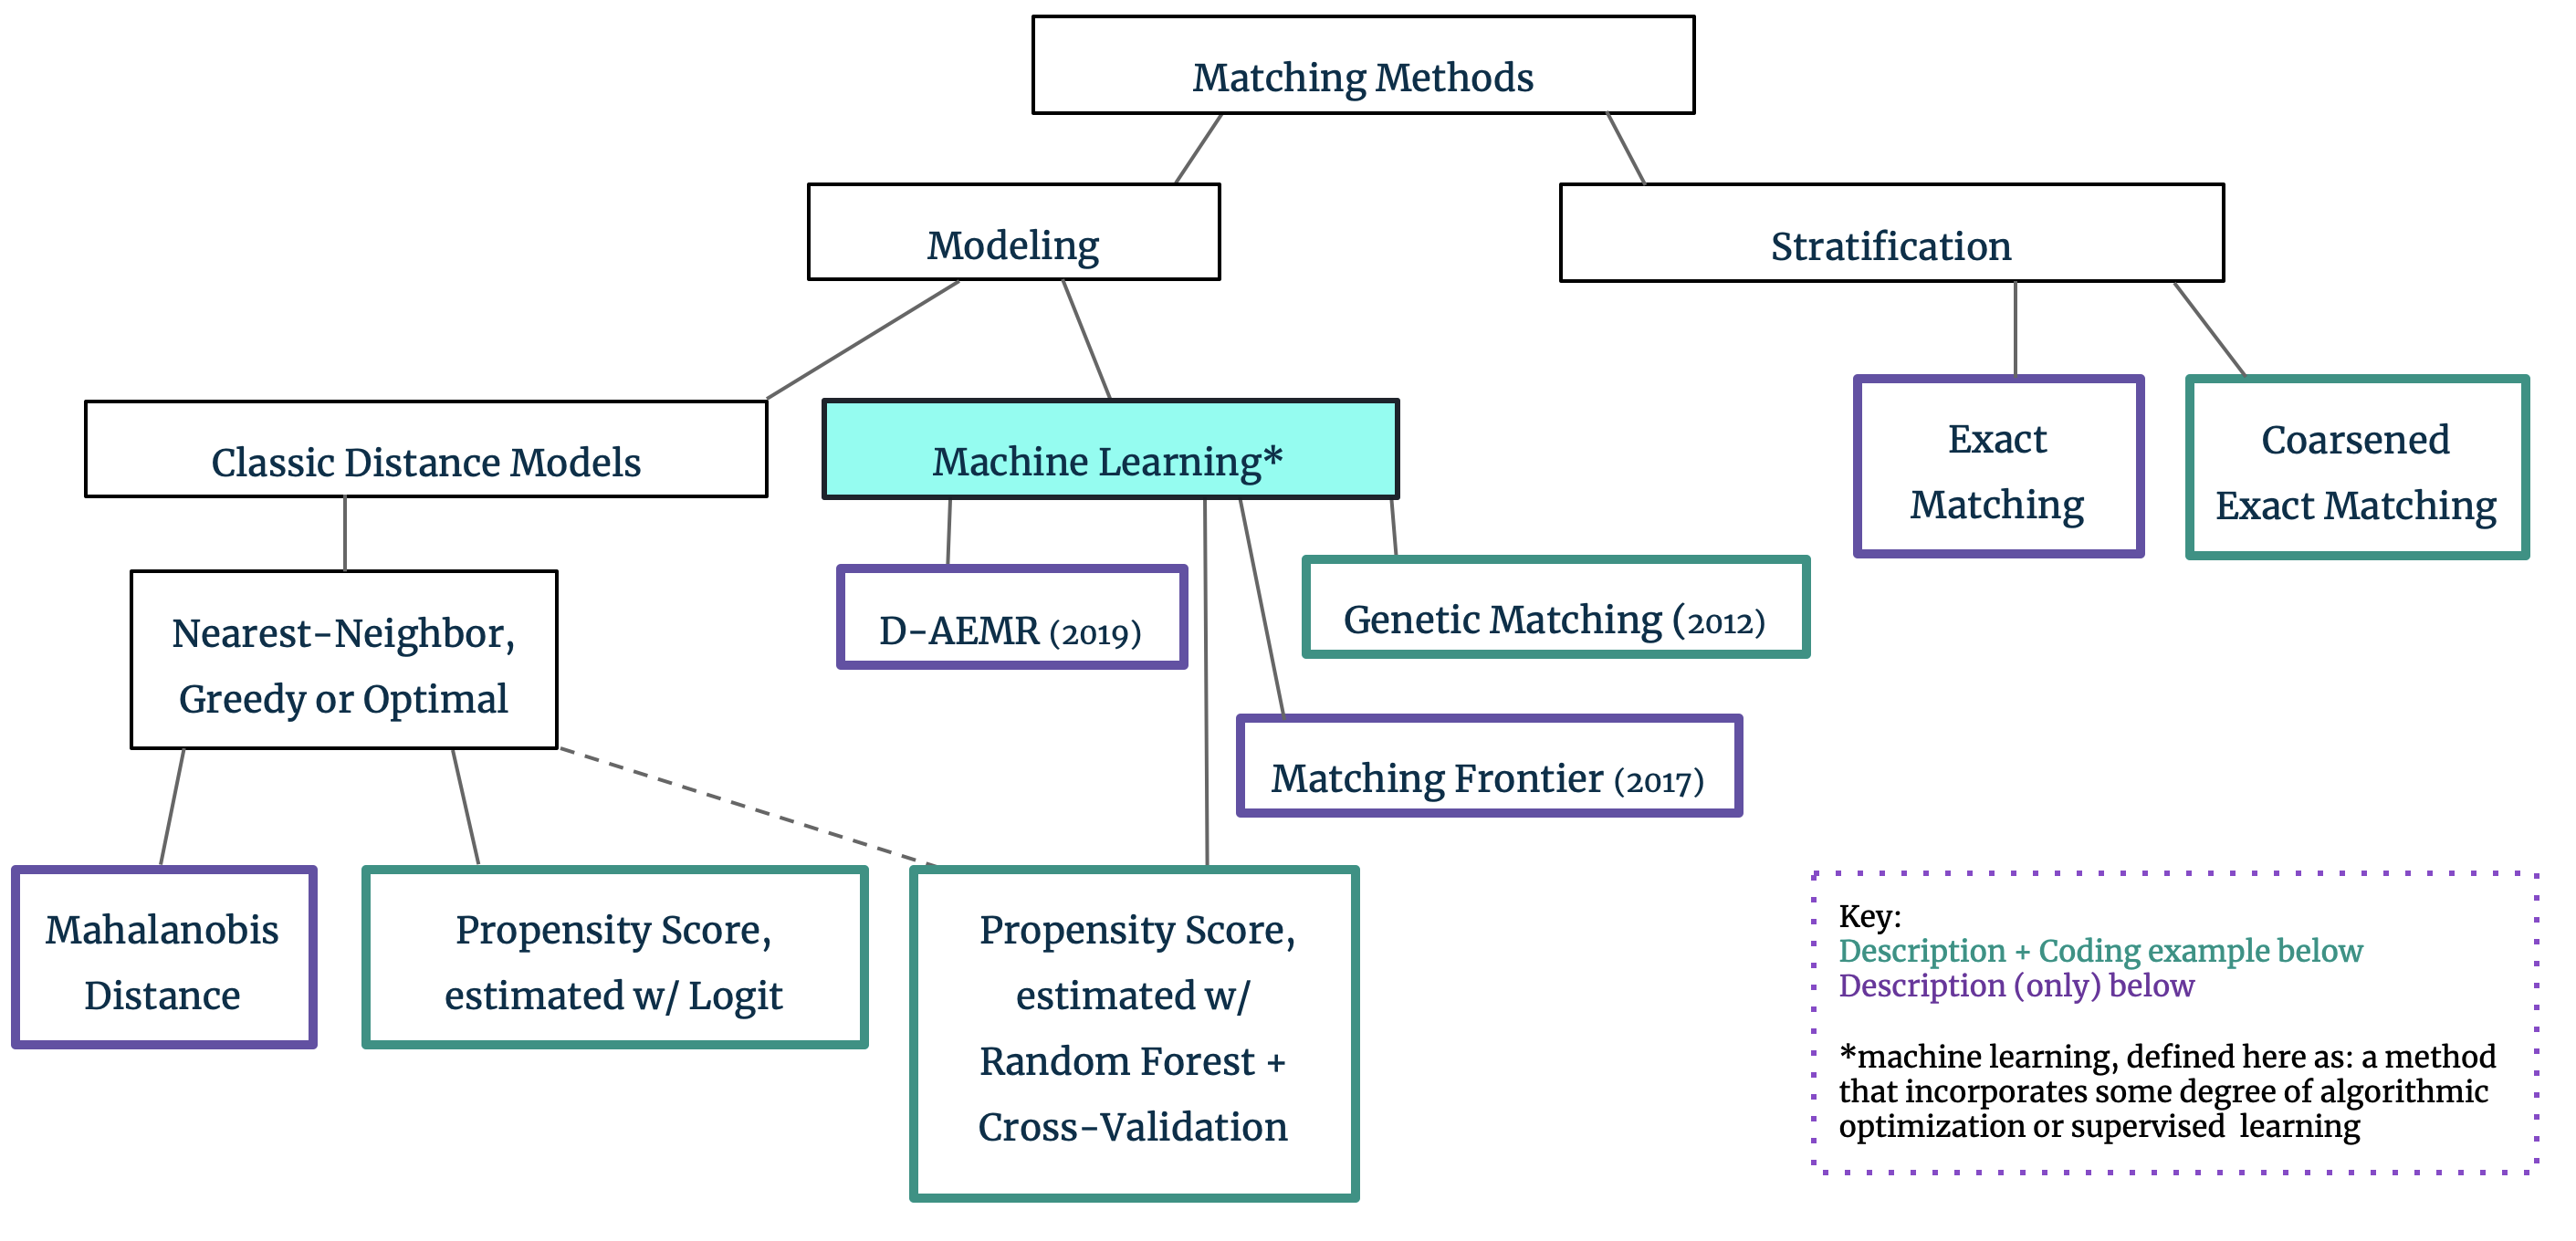
\includegraphics[width=\textwidth]{images/matching-methods.png}\\[2\baselineskip]
{\color{Gray}
{\tiny Authors: Samantha Sizemore and Raiber Alkurdi\\[0.25\baselineskip]
{\itshape Matching Methods For Causal Inference: A Machine Learning Update}\\[-0.75\baselineskip]
\texttt{https://humboldt-wi.github.io/blog/research/applied\_predictive\_modeling\_19/matching\_methods/}
}
}

\end{frame}

%------------------------------------------%
% History of Nearest Neighbor Search
%------------------------------------------%

\begin{frame}{The History of Nearest Neighbor Search}

\begin{minipage}{0.6\textwidth}

\small

\begin{itemize}

\vspace{0.5\baselineskip}

\item {\bfseries Literate Programming}

\vspace{0.25\baselineskip}

{\itshape ``Instead of imagining that our main task is to instruct a computer what to do, let us concentrate rather on explaining to {\bfseries human beings} what we want a computer to do.''}

\vspace{-0.5\baselineskip}
\begin{flushright}
{\footnotesize - Donald Knuth}
\end{flushright}

\item {\bfseries Analysis of algorithms }

The study of the complexity of algorithms.

\vspace{0.5\baselineskip}
\item Creator of the {\bfseries \TeX}!

\end{itemize}

\end{minipage}\hspace{0.05\textwidth}%
\begin{minipage}{0.3\textwidth}

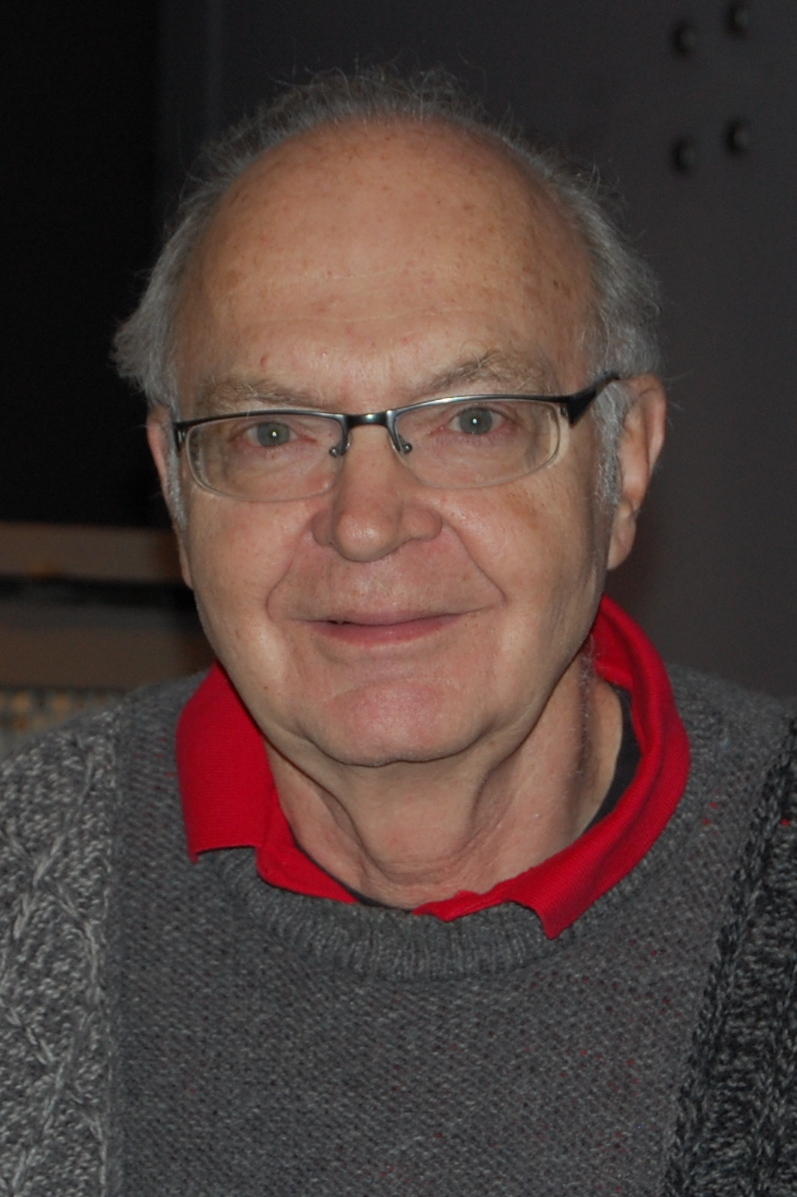
\includegraphics[width=\textwidth]{images/knuth.jpg}
\vspace{-0.5\baselineskip}

{\footnotesize {\bfseries Donald Knuth}} \tiny \\Computer History Museum's Revolution Exhibition (2011)\\[0.5\baselineskip]
{\color{Gray}
Author: Alex Handy\\[0.125\baselineskip]
CC BY-SA 2.0\\[0.125\baselineskip]https://creativecommons.org/licenses/by-sa/2.0}
\end{minipage}

\end{frame}


%------------------------------------------%
% k-Nearest Neighbor Search
%------------------------------------------%

\begin{frame}{Modern Search Algorithms}

\small

%\vspace{-1\baselineskip}
\begin{itemize}

\item {\bfseries $k$-NN search} - Find the $k$ closest points to point $P$.

\begin{itemize}

\vspace{0.25\baselineskip}
\item PCA into feature space, followed by k-NN classification.

\end{itemize}

\vspace{0.75\baselineskip}
\item {\bfseries Mahalanobis distance} - a measure of the distance between a point $P$ and a distribution $D$.

{\tiny Hypothetical 2D example of Mahalanobis distance.}

\begin{minipage}{0.65\textwidth}

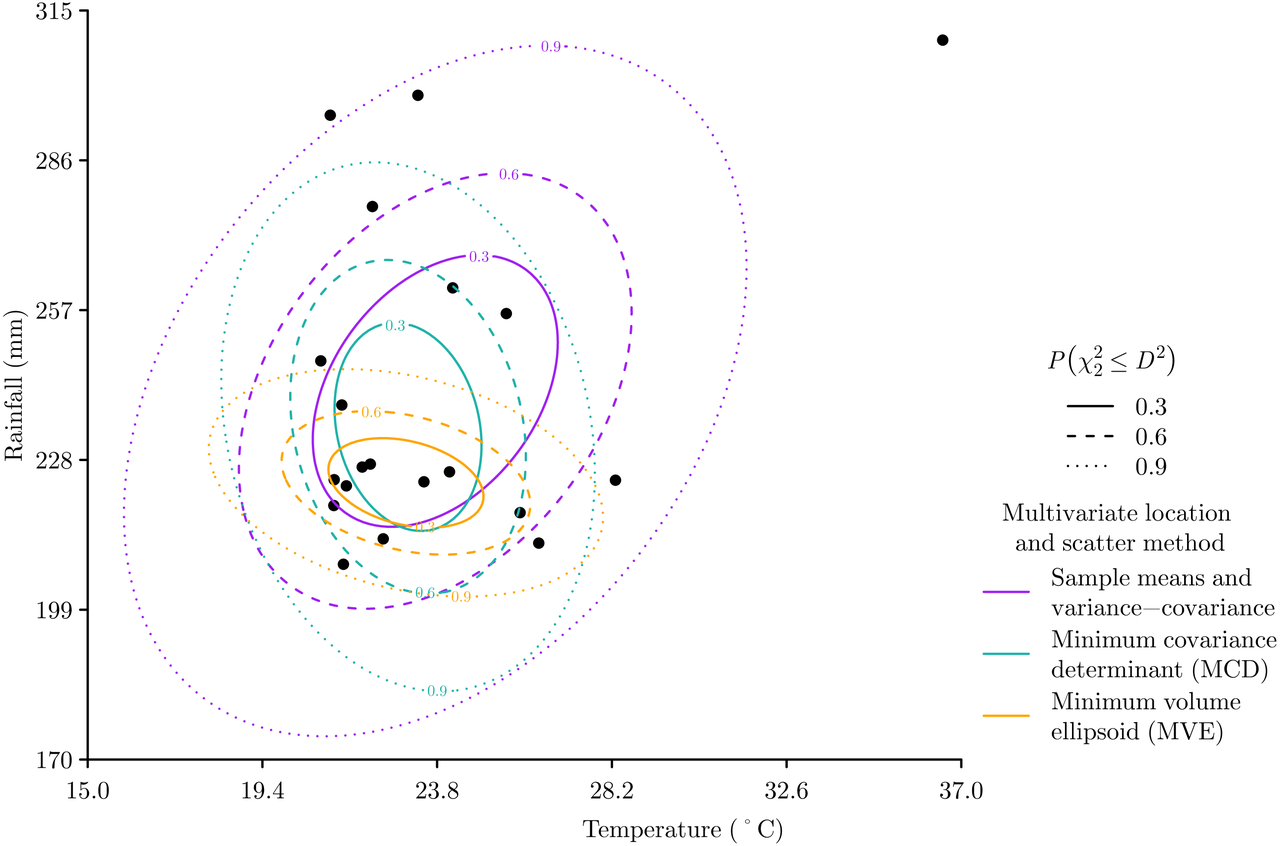
\includegraphics[width=\textwidth]{images/mahalanobis-distance.png}

\end{minipage}\hspace{0.00\textwidth}%
\begin{minipage}{0.25\textwidth}

\vspace{-8\baselineskip}

{\tiny {\color{Gray} Author:\\[-0.5\baselineskip]Tretherington\\[-0.5\baselineskip]
CC BY-SA 4.0\\[-0.5\baselineskip]https://creativecommons.org \\[-0.5\baselineskip]/licenses/by-sa/4.0}
}

\end{minipage}

%\vspace{0.75\baselineskip}
%\item {\bfseries Propensity score matching (PSM)} - Estimate the effect of a treatment by accounting for the covariates that predict receiving the treatment.

\end{itemize}

\end{frame}

% https://en.wikipedia.org/wiki/Mahalanobis_distance
% https://en.wikipedia.org/wiki/Propensity_score_matching
% https://en.wikipedia.org/wiki/Nearest_neighbor_search


%------------------------------------------%
% k-Nearest Neighbor Search
%------------------------------------------%

\begin{frame}{Supervised learning}

{\bfseries Supervised learning} is task of learning a function that maps an input to an output based on example input-output pairs.

\vspace{1\baselineskip}
\begin{enumerate}

\item Infer a function from labeled training data.

  \begin{itemize}
  
  \vspace{0.5\baselineskip}
  
  \item Use training examples to get training data.
  
  \vspace{0.5\baselineskip}
  
  \item Each example is a pair of an input object and a desired output value, e.g. $(\text{"}\Delta \text{--9 THC"}, \text{ "delta\_9\_thc"})$.

  \end{itemize}

\vspace{0.75\baselineskip}

\item Map new examples.

  \begin{itemize}
  
    \vspace{0.5\baselineskip}
  \item Generalize from the training data to unseen situations.  
  
  \end{itemize}

\vspace{0.75\baselineskip}

\item Re-train the model with new training examples.

\end{enumerate}

\vspace{\baselineskip}
{\small
{\bfseries Goal:} Correctly determine the class labels for unseen instances.
}
\end{frame}


%------------------------------------------%
% Application
%------------------------------------------%

\begin{frame}{Cannabis Data Science Application}

\begin{center}
\begin{minipage}{3.85in}

\begin{center}
\begin{minipage}{\linewidth}
\begin{Block}{Cannabis Data Science Application}

\vspace{0.5\baselineskip}

\begin{itemize}

\item Can we use {\bfseries matching models} to find cannabis products similar to a given product?

\vspace{0.75\baselineskip}

\end{itemize}

\end{Block}
\end{minipage}
\end{center}

\vfill

\end{minipage}
\end{center}

\end{frame}

%------------------------------------------%
% Takeaway
%------------------------------------------%
\section{Takeaway}

\begin{frame}{}

\vspace{0.5\baselineskip}

\begin{center}
\begin{minipage}{3.85in}

% Thank you.

\includegraphics[width=.25in]{images/prayer.png} {\Large \textbf{Thank you for coming.}}\\[-0.75\baselineskip]

\begin{center}
\begin{minipage}{\linewidth}
\begin{Block}{Insights of the Day}

\vspace{0.5\baselineskip}

\begin{itemize}

\item Small, seemingly inconsequential actions can have profound long-term effects because of {\bfseries \underline{compounding}}.

\vspace{0.75\baselineskip}

\end{itemize}

\end{Block}
\end{minipage}
\end{center}

\vfill

\end{minipage}
\end{center}

\vspace{0.5\baselineskip}

{\large What is on your mind for next week?}\\

\end{frame}


%------------------------------------------%
% Fin.
%------------------------------------------%
\end{document}
